\documentclass{ecai}
\usepackage{times}
\usepackage{graphicx}
\usepackage{latexsym}
\usepackage{xcolor}
\usepackage{relsize}
\usepackage{hyperref}
%%% call for papers: http://ecai2020.eu/call-for-papers/mainconference/
\ecaisubmission   % inserts page numbers. Use only for submission of paper.
                  % Do NOT use for camera-ready version of paper.

\newcommand{\RefPerSys}{{\textit{\textsc{RefPerSys}}}}

% defines the \rpsgitcommit command:
\input{generated-ecai2020-gitid}
\begin{document}

\title{Development and Architecture of {\RefPerSys}\\ {\relsize{-1}{A
      Multi-Threaded \textsc{Ref}lective \textsc{Per}sistent \textsc{Sys}tem} for AI}}

\author{Basile Starynkevitch\institute{Bourg La Reine, France, email: \href{mailto:basile@starynkevitch.net}{\texttt{basile@starynkevitch.net}}}
\and Abhishek Chakravarti \institute{Kolkata, India, email: \href{mailto:chakravarti.avishek@gmail.com}{\texttt{chakravarti.avishek@gmail.com}}}
\and  Nimesh Neema\institute{Indore, India, email: \href{mailto:nimeshneema@gmail.com}{\texttt{nimeshneema@gmail.com}}}\\
\href{http://refpersys.org/}{\texttt{refpersys.org}}}

\maketitle
\bibliographystyle{ecai}

\begin{abstract}
  %% TODO: REWRITE ABSTRACT not scientific enough.
  %\textcolor{red}{REWRITE THIS}
  
  %\textsc{\textbf{RefPerSys}} is a \textsc{\textbf{Ref}}lexive and orthogonally 
  %\textsc{\textbf{Per}}sistent \textsc{\textbf{Sys}}tem (as a GPLv3+ licensed 
  %free software running on Linux; it is a still unfunded research project 
  %expected to last for many years, with the aim of experimenting
  %with open science ideas close to Artificial General Intelligence dreams. This
  %starting project is notably inspired by the works of J. Pitrat (see 
  %\cite{Pitrat:2009:ArtifBeings, Pitrat:1996:FGCS, Pitrat:2009:AST, Pitrat:blog}).

The technical progress of computing hardware, especially with the prevalence of
multicore systems and large amounts of RAM, now allows us to further experiment
with the Artificial General Intelligence goals inspired by the works of pioneers
such as J. Pitrat\cite{Pitrat:2009:ArtifBeings, Pitrat:1996:FGCS, Pitrat:2009:AST}.
Our project is exploring the development, through the use of metaprogramming approaches,
a bootstrapped multithreaded, reflexive and orthogonally persistent Quine system running
on modern Linux x86-64 hardware, leading to a declarative knowledge-based language.
\end{abstract}

\smallskip

\textbf{Topics :} Knowledge Representation and Reasoning, Machine
Learning, Multidisciplinary Topics and Applications, Agent-based and
Multi-agent Systems, Semantic Technologies.

\medskip

\section{MOTIVATIONS}
\label{sec:motivations}

A symbolic AI software system running on \textsc{Linux} nowadays needs to
manage a large amount of information and knowledge organized as some
complex graph (also known as an \emph{ontology}
\cite{DeNicola:2009:OntologyBuilding}, a \emph{semantic network}
\cite{VanDeRiet:1992:Ling-instr-know}, or a \emph{frame}
%%
%\cite{Bobrow-Winograd:1977:KRL, greiner:1980:representation,
%  Lenat:1983:Eurisko, Lenat:1983:theory, Lenat:1991:ev-cycl}) inside
%%
\cite{Bobrow-Winograd:1977:KRL, Lenat:1983:theory}) inside the
computer memory. This large graph should be orthogonally persistent
\cite{Dearle:2010:orthopersist} (such as in \textsc{Bismon}
\cite{Starynkevitch:2019:bismon-draft}) on disk, and be loaded from
files at startup time on mornings of worked days, and later dumped to
disk, as a set of \emph{state files} in \href{http://hjson.org/}{\textsc{Hjson}} format, before
normal termination when leaving office at evening. Having these files
in a textual format facilitates their management with existing
distributed version control systems such as
\href{http://git-scm.com}{\texttt{git}} or software development forges
like \href{http://gitlab.com/}{\texttt{gitlab}} and ensures some data
portability. Carefully generating the runtime, through metaprogramming
approaches, as \emph{C++} code (à la \textsc{Gcc Melt}
%%
%\cite{Starynkevitch-DSL2011, Starynkevitch:2009:grow,
  %Starynkevitch:2007:Multistage} or \textsc{Bismon}) that is subsequently compiled by
  %%
\cite{Starynkevitch-DSL2011} that is subsequently compiled by
  %Starynkevitch:2007:Multistage} or \textsc{Bismon}) that is subsequently compiled by
\texttt{g++} into \texttt{dlopen}-ed plugins\footnote{In practice, as
demonstrated by the \texttt{manydl.c} sample code written for J. Pitrat, on
\href{http://github.com/bstarynk/misc-basile/}{\texttt{github.com/bstarynk/misc-basile/}},
several hundreds of thousands of \texttt{*.so} plugins can be
generated and then dynamically loaded by \texttt{dlopen} at runtime on
\textsc{Linux} desktops.} provides some amount of code portability. Current
desktop computers are powerful enough to keep a large memory heap in
%%
%RAM\footnote{Notice that the C++ source of software (such as the
%\textsc{Gcc} compiler, the \textsc{Qt} GUI toolkit, or the
%\textsc{PostGreSQL} database) made of millions of lines of code fits
RAM\footnote{Notice that the millions of SLOC for mature software (such as the
\textsc{Gcc} compiler, the \textsc{Qt} GUI toolkit, or the
\textsc{PostGreSQL} database), fits entirely in the 64 GB RAM of a powerful desktop. 
But compiling such a code base takes hours of computer time.}, and this entire heap
%%
%can be persisted on disk, in a manner similar to relational database management systems
%\cite{levene:2012:relational-databases} such as
%\href{http://sqlite.org/}{\textsc{Sqlite}} or \textit{NoSQL} databases
%\cite{RAJ-2018-NoSQL} do. 
can be persisted on disk, similar to how database management systems
%\cite{levene:2012:relational-databases} such as
%\href{http://sqlite.org/}{\textsc{Sqlite}} or \textit{NoSQL}\cite{RAJ-2018-NoSQL} work. 
such as \href{http://sqlite.org/}{\textsc{Sqlite}} or \href{https://en.wikipedia.org/wiki/NoSQL}{\textit{NoSQL}} work. 

Current processors are multi-core, so running a good enough multi-threaded program on them
\cite{butenhof:1997:programming} should be beneficial for
performance. Backtracing libraries such as I. Taylor's
\href{https://github.com/ianlancetaylor/libbacktrace}{\texttt{libbacktrace}}
facilitate introspection of the current thread's call stack, if the
\emph{C++} code has been compiled, using \texttt{g++ -O2 -g}, with
\textsc{Dwarf} debugging information. JIT-compiling libraries (such as
\href{https://gcc.gnu.org/onlinedocs/jit/}{\texttt{libgccjit}}) can
produce plugins without the need of a textual representation of some
\href{https://en.wikipedia.org/wiki/Abstract_syntax_tree}{AST} of the
code.


%%%%%%%%%%%%%%%%%%%%%%%%%%%%%%%%%%%%%%%%%%%%%%%%%%%%%%%%%%%%%%%%

\section{THE {\RefPerSys} ROADMAP}
\label{sec:roadmap}

\subsection{A Staircase Development Model}
\label{subsec:stairecase}

%% copied text and figure from refpersys-design.tex & spiral-stairs.svg
{\RefPerSys} development model is similar to a staircase, as depicted
%in figure \ref{fig:bootstrap-stair}. It is different from the
%traditional spiral development model \cite{boehm:1988:spiral}. The
in Figure \ref{fig:bootstrap-stair}, unlike the traditional spiral development
model \cite{boehm:1988:spiral}. The
%initial
floor of the staircase is just a C++ hand-coded persistent
system, and we gradually add new code implementing more features
(first entirely hand-written, later more and more parts of it being replaced
by {\RefPerSys} generated code). We are progressively replacing
existing hand-written code (or low-level DSL) by more a expressive and
generated one. So we will continuously rewrite past formalizations as
more clever and expressive ones, taking increasing advantage of
{\RefPerSys} %whole-system 
system-wide introspective and metaprogramming abilities.


\begin{figure}[h]
  \begin{center}
    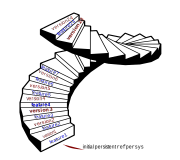
\includegraphics[width=0.32\textwidth]{spiral-stairs}
  \end{center}

  \begin{quote}
    \begin{relsize}{-0.4}
    Each new feature -or small incremental change or a few of them
    (small \texttt{git commit}s) - of {\RefPerSys} enables us to build
    and \textbf{generate} the next version of {\RefPerSys}, and a next
    feature is then added to that \textit{improved} version, and so on
    repeatedly, etc....
    \end{relsize}
  \end{quote}
  
  \caption{the strange \textbf{{\RefPerSys} staircase development model} {\relsize{-1}{(from a \href{https://thenounproject.com/term/spiral-stairs/956427/}{figure of Spiral stairs} by Lluisa Iborra from the Noun Project)}}}
  \label{fig:bootstrap-stair}
\end{figure}

So the {\RefPerSys} project is taking a bootstrapping approach
\cite{Pitrat:1996:FGCS, Pitrat:2009:ArtifBeings,
  hernandez-phillips:2019:debugging-bootstrap} : progressively old
code (perhaps even hand-written, or generated) is replaced by
``better'' code emitted by metaprogramming techniques from higher
level formalizations.

%%%%%%%%%%%%%%%%
\subsection{Initial Architecture of \RefPerSys}
\label{subsec:initarchi}

The initial architecture\footnote{The GPLv3+ code of \textsc{Bismon},
mostly in C, is available on
\href{https://github.com/bstarynk/bismon/}{\texttt{github.com/bstarynk/bismon/}}. But
     {\RefPerSys} is coded in C++, only for \textsc{Linux/x86-64}, on
     \href{https://gitlab.com/bstarynk/refpersys}{\texttt{gitlab.com/bstarynk/refpersys}}
     and share almost no code with \textsc{Bismon}.}, prototyped in
C++17, of {\RefPerSys} is close to \textsc{Bismon}'s one. But it
should evolve very differently. Our persistent and garbage-collected
\cite{jones:2016:gchandbook} heap is made of \emph{values}. Most
values are immutable and rather light. Some values are mutable
\emph{objects}, which are quite heavy, since synchronized between
threads so carrying their read-write lock. Values are represented in
64 bits machine words: either a tagged integer, or containing a
pointer to some aligned memory zone. Most values are persistent---so
dumped then later reloaded through state files---but some are transient,
since it makes no sense to keep them on disk. Transient values, often
transient objects, include reification of GUI windows or Web widgets,
HTTP connections, ongoing processes, in particular compilation
commands of newly generated plugins, etc.. Values are both ordered
and hashable, so fit nicely inside standard C++ containers like
\texttt{std::set} or \texttt{std::unordered\_map}. Every mutable
object has a globally unique, fixed, and random \emph{objid}, which
fits in 16 bytes and is textually represented---in state files---with a
string such as \texttt{\_7VnQtHZ63pA02rCekc}.

Immutable values include \textsc{Utf-8} strings, boxed \textsc{Ieee}
64 bits floats without \texttt{NaN} to stay ordered, tuples of
references to objects, ordered sets of objects, closures -whose code
is represented by some object, and with arbitrary values as closed
values-, and immutable instances.

Mutable objects carry their constant \emph{objid}, their lock, their
class -which could change at runtime and is an object-, attributes,
components, and some optional smart \texttt{std::unique\_ptr} pointer
to the payload of that object. An attribute associates a key -itself
some object reference- to a value, so attributes are collected in some
mutable C++ \texttt{std::map}. The components are organized as a
\texttt{std::vector} of values. The payload belongs to its owning
object and carry extra data, such as mutable hashed sets, class
information -sequence of superclasses and method dispatch table-,
string buffers, opened file or socket handles, GUI or widgets etc..

%%%
%The initial {\RefPerSys} should contain some ad-hoc integrated
%development environment above the \textsc{Fltk} toolkit, used just to
%fill the persistent heap and generate some of its C++ code.
%%%
{\RefPerSys} will initially have an ad-hoc IDE---built with the \textsc{Fltk}
toolkit---to just fill the persistent heap and generate some of its C++
code. This IDE will support the syntax highlighting, autocompletion and
navigating of objects through their \emph{objids}.

%%%%%%%%%%%%%%%%%%%%%%%%%%%%%%%%%%%%%%%%%%%%%%%%%%%%%%%%%%%%%%%%%%%%%%

\section{METAPROGRAMMING IN \RefPerSys}
\label{sec:metaprogramming}

An essential insight of {\RefPerSys} is metaprogramming, practically
done by generating \emph{C++17} code at runtime for a Linux
system. This is strongly inspired by previous work, see
\cite{Pitrat:1996:FGCS, Pitrat:2009:ArtifBeings,
  Starynkevitch:2019:bismon-draft, Starynkevitch-DSL2011,
  Starynkevitch:2007:Multistage}. The choice of the actual programming
language used to generate code\footnote{In practice, some C++ code is
emitted in a file similar to \texttt{/tmp/generated.cc}, compiled as a
plugin by forking \texttt{g++ -O -g -fPIC -shared} into a
\texttt{/tmp/generated.so}, which is later \texttt{dlopen}-ed, all by
the same process running the \texttt{./refpersys} executable.} in
within {\RefPerSys} is mostly arbitrary and guided by non-technical
concerns: which programming language is known to all the {\RefPerSys}
team, while being compatible with a lot of existing open source
libraries and APIs? That programming language happens to be C++
(better than C, because of its containers; also used in
\href{http://tensorflow.org}{\textsc{TensorFlow}} or
\href{https://gudhi.inria.fr/}{\textsc{Ghudi}}), but our expansion
machinery is inspired by \textsc{Melt} code chunks
\cite{Starynkevitch-DSL2011}, \textsc{Lisp} macros
\cite{Queinnec:1996:LSP} or \textsc{Django} templates, driven by
``expert system''-like meta rules (such as in \cite{Pitrat:1996:FGCS})
potentially applicable to themselves.


%\textcolor{red}{TO BE WRITTEN}

\bigskip

\section{CONCLUSION}
We have discussed how we are trying to develop {\RefPerSys} organically,
using metaprogramming techniques to eventually build a fully bootstrapped
Quine system. Our approach is to gradually replace hand-written code with
increasingly expressive generated code, relying on the growing metaprogramming
and reflective properties of the system. See also \cite{starynkevitch:2019:refpersys-design}.

%%%%%%%%%%%%%%%%%%%%%%%%%%%%%%%%%%%%%%%%%%%%%%%%%%%%%%%%%%%%%%%%%%%%%%
\ack Thanks to François Bancilhon for proof-reading this draft.

\bibliography{../bib-refpersys}

%%% for a draft that should be acceptable
\begin{flushright}
  \begin{relsize}{-1}
    Our draft \texttt{git} ID is \texttt{\textit{\rpsgitcommit}}
  \end{relsize}
\end{flushright}

\end{document}
%%%%%%%%%%%%%%%%%%%%%%%%%%%%%%%%%%%%%%%%%%%%%%%%%%%%%%%%%%%%%%%%%%%%%%

%%% For emacs:
%%%%%%%%%%%%%%%%%%%%%%%%%%%%%%%%%%%%%%%%%%%%%%%%%%%%%%%%%%%%%%%%
%% Local Variables: ;;
%% compile-command: "./build.sh" ;;
%% End: ;;
%%%%%%%%%%%%%%%%%%%%%%%%%%%%%%%%%%%%%%%%%%%%%%%%%%%%%%%%%%%%%%%%
